\documentclass{sigchi}


%% EXAMPLE BEGIN -- HOW TO OVERRIDE THE DEFAULT COPYRIGHT STRIP -- (July 22, 2013 - Paul Baumann)
\toappear{
{\emph{CS262A}}, Fall 2014, Berkeley, CA, USA. \\
Copyright is held by the owner/author(s).  \\
http://expresso.cearto.com}
%% EXAMPLE END -- HOW TO OVERRIDE THE DEFAULT COPYRIGHT STRIP -- (July 22, 2013 - Paul Baumann)


% \pagenumbering{arabic}
\usepackage{balance}  % to better equalize the last page
\usepackage{graphics} % for EPS, load graphicx instead
\usepackage{times}    % comment if you want LaTeX's default font
\usepackage{url}      % llt: nicely formatted URLs
 \newtheorem{theorem}{Theorem}
 \newtheorem{lemma}[theorem]{Lemma}

% llt: Define a global style for URLs, rather that the default one
\makeatletter
\def\url@leostyle{%
  \@ifundefined{selectfont}{\def\UrlFont{\sf}}{\def\UrlFont{\small\bf\ttfamily}}}
\makeatother
\urlstyle{leo}


% To make various LaTeX processors do the right thing with page size.
\def\pprw{8.5in}
\def\pprh{11in}
\special{papersize=\pprw,\pprh}
\setlength{\paperwidth}{\pprw}
\setlength{\paperheight}{\pprh}
\setlength{\pdfpagewidth}{\pprw}
\setlength{\pdfpageheight}{\pprh}
\usepackage[ruled,vlined]{algorithm2e}
% Make sure hyperref comes last of your loaded packages, 
% to give it a fighting chance of not being over-written, 
% since its job is to redefine many LaTeX commands.
\usepackage[pdftex]{hyperref}
\hypersetup{
pdftitle={Expresso: Perceptual Scheduling for Embedded Systems},
pdfauthor={Cesar Torres},
pdfkeywords={SIGCHI, proceedings, archival format},
bookmarksnumbered,
pdfstartview={FitH},
colorlinks,
citecolor=black,
filecolor=black,
linkcolor=black,
urlcolor=black,
breaklinks=true,
}
\DeclareMathOperator{\dis}{d}
\newcommand\tabhead[1]{\small\textbf{#1}}
\newcommand{\expresso}{ExPRESSO }
%\newcommand*{\layer}[1]{{\sffamily{#1}}}
%\newcommand*{\layer}[1]{{\textit{#1}}}
%\newcommand*{\layer}[1]{{\texttt{#1}}}
\newcommand*{\schedule}[1]{{\textbf{\small{\fontfamily{cmss}\selectfont{#1}}}}}
% set up tight list spacing
\usepackage{enumitem} 
\setlist{nolistsep,nosep}

% for toggles
\usepackage{etoolbox}


% CHANGE FROM TOGGLE TRUE TO TOGGLE FALSE FOR NON-ANONYMOUS RENDERING
% http://tex.stackexchange.com/questions/5894/latex-conditional-expression
\newtoggle{anonymous}
% \toggletrue{anonymous}
\togglefalse{anonymous}

% CHANGE FROM TOGGLE TRUE TO TOGGLE FALSE TO HIDE COMMENTS
\newtoggle{comments}
%\toggletrue{comments}
\togglefalse{comments}

% Comment region command (from Wesley Willett)
\usepackage[usenames]{color}
\usepackage[usenames,dvipsnames]{xcolor}
\iftoggle{comments} {
  %if we want to show comments
  \newcommand {\tim}[1]{{\color{magenta}\bf{TC: #1}\normalfont}}
  \newcommand {\cesar}[1]{{\color{NavyBlue}\bf{CT: #1}\normalfont}}
  \newcommand {\ep}[1]{{\color{violet}\bf{EP: #1}\normalfont}}
  \newcommand {\bjoern}[1]{{\color{Orange}\bf{BH: #1}\normalfont}}
  \newcommand {\savage}[1]{{\color{Blue}\bf{VS: #1}\normalfont}}
}{
  %if we don't want to show comments
  \newcommand {\tim}[1]{}
  \newcommand {\harper}[1]{}
  \newcommand {\ep}[1]{}
  \newcommand {\bjoern}[1]{}
  \newcommand {\savage}[1]{}
  \newcommand {\cesar}[1]{}
}

 
\begin{document}

\title{\expresso: Perceptual Scheduling for Embedded Systems}

\iftoggle{anonymous}{
  %if anonymous
  \numberofauthors{1}
  \author{
  \alignauthor Anonymous for Submission\\
    \affaddr{...}\\
    \affaddr{...}\\
    \email{...}\\
  }
}{
\numberofauthors{1}
  \author{
  \alignauthor {C\'{e}sar Torres}\\
    \affaddr{Department of Electrical Engineering and Computer Sciences}\\
    \affaddr{University of California Berkeley}\\
    \email{cearto@eecs.berkeley.edu}\\
  }
}
\maketitle
\section{Abstract}
  Actuators in embedded systems are conventionally used in simple, yet limited ways --- usually bound to a binary state or mapped to a sensor value. However, there exists a wide design space that can enhance a system's ability to communicate to a user. As more Internet of Things devices enter this landscape, the ability to control several actuators is limited by both the performance constraints of the embedded system and the current scheduling routines which require precisely timed signals for each actuator in the system. We introduce the \expresso Perceptual Scheduler (\schedule{EPS}), a mechanism which factors in the different mechanical, perceptual, and software (MPS) profiles of actuators within a system to produce perceptually accurate and synchronous output. We show how \schedule{EPS} is able to operate on a portion of system bandwidth and still maintain the quality of service of its perceptual tasks while degrading gracefully under oversubscription. 



\keywords{Scheduling, Internet of Things, perception}
\category{H.5.m.}{Information Interfaces and Presentation (e.g. HCI)}{Miscellaneous}
\section{Introduction}

  % the heterogeneity of different types of modalities such as motion, heat, light, sound in an actuator system. 
  % the difsingle-threaded environment and hardware's capability to handle  and the task of coordinating actuator behaviors is conceptually constrained by interleaving commands. This project introduces a perceptual scheduling mechanism which factors in the different mechanical, perceptual, and software (MPS) profiles of actuators. We show that this improves perceptual performance and degrades gracefully under different hardware constraints. 

  In physical computing, tasks which require physical output to convey information, which we term behaviors, are subject to a different type of constraints than traditional software tasks. These types of tasks are subject to both mechanical impedances of the actuator mechanisms as well as discrepancies between physical stimuli and the human perceptual system. In this paper, we show how this is further complicated when systems are required to control actuation of several modalities (light, heat, angle, vibration) at scale. 


    \begin{figure}[t]
      \centering
      \includegraphics[keepaspectratio, width=0.47\textwidth]{figures/system.pdf}
      \caption{ The ExPRESSO pipelines consists of a content creation stage with stores content in a SQL db. This is then called-on-demand by the scheduler, where it is then compiled and sent as actuation tasks to micro controllers in a actuator system, who then handle routing commands to the appropriate actuators. }
        \label{fig:system} 
    \end{figure}

 Behaviors have already been shown to be incredibly successful at conveying system state \cite{harrison_unlocking_2012,kuznetsov_red_2011}. Such examples include Huppi et. al. patented ``breathing'' status LED indicator used in modern Apple computers \cite{huppi_breathing_2003}, or the 8-bit sound aesthetic from early gaming systems \cite{kaliakatsospapakostas_interactive_2012}. 
 However, as the number of distributed wireless-addressable actuators in the Internet of Things (IoT) increases, e.g., Phillips Hue lights, new types of \textit{distributed} behaviors arise, or behaviors which take into consideration the environment and each other, rather than operating as point-based designs. 

Developing distributed behaviors can enable ambient display technologies, such as ambientROOM, an environment which uses ambient media –-- ambient light, shadow, sound, airflow, water flow --- to communicate information in the cognitive-background, opening a new interaction space where users can transition between background and foreground information \cite{ishii_tangible_1997}. Furthermore, controlling distributed actuators at scale has been show to enable ad-hoc display technologies. For instance, Schwarz et. al. demonstrates how localizing cell phone screens in a scene and controlling their output can be used to construct large collective displays in situations like sporting events, concerts and political rallies \cite{schwarz_phone_2012}. Heaton similarly shows how distributed devices disrupt the current paradigm of ``matrix'ed" displays, and redefine control of both a pixel (data structure) and the physical pixel (visible form)\cite{heaton_physical_2000}.

This vision however is currently limited by performance constraints (I/O-bound) of embedded systems and current scheduling routines which require precisely timed signals for \textit{each} actuator in the system --- restricting the scalability of the system. Furthermore, for a distributed actuator system (DAS), every node has a different performance profile and network latency, which make coordinating behaviors especially difficult \cite{ballagas_patch_2004}. 


These issues are currently mediated through hardware optimizations. For example, LED drivers use a shared common hardware line and multiplexed signals to drive multiple LEDs in parallel. This takes advantage of driving a single common actuator, and foregoes the complexities of controlling systems with multiple actuators. Recent advancements in LED driver firmware such as Fadecandy \cite{scott_fadecandy_2013} circumvent creating precisely timed signals by using perceptual optimizations such as dithering and color correction. However, hardware-centric techniques, while powerful for controlling large sets of connected actuators, are bound by the physical constraints of hardware lines. 

Currently within embedded systems, software-controlled behaviors are interrupt-driven, a preemptive approach that at scale can reduce the performance of the system. Alternatively, these behaviors are manually programmed by interleaving commands, a tedious and conceptually-restrictive process which does not fit into an iterative design practice. 
 
In this paper, we extend the definition of a perceptual scheduler \cite{chaudhary_perceptual_2001} to apply to distributed actuator systems. Firstly, we describe a Perceptual Task (PT) compiler , which uses the different mechanical, perceptual, and software (MPS) profiles of actuators to convert high resolution tasks into perceptually accurate, correct, and synchronous output. 

We introduce the \expresso Perceptual Task Scheduler (\schedule{PTS}), a scheduling mechanism which factors a perceptual model that utilized principles from psychophysics literature \cite{pelli_psychophysical_1995}, as well as Gestalt psychology. We show how it is able to operate on a portion of system bandwidth by extending Abeni's et.al. work on Constant Bandwidth Server (CBS) \cite{abeni_integrating_1998}, to incorporate a temporal dithering technique and a perceptual saliency queue. Together, the PT compiler and the \schedule{PTS} mechanism demonstrates a full pipeline for enabling distributed behaviors. 

Lastly, we define an perceptual error metric that can be used to evaluate the perceptual quality of the output. Using a synthetic macrobenchmark, we demonstrate that the \schedule{PTS} mechanism is able to maintain the quality of service (QoS) of its perceptual tasks over different hardware profiles, while degrading gracefully under oversubscription. 

\section{BACKGROUND}

  \subsection{Scheduling}
  The CBS algorithm \cite{abeni_integrating_1998} provides certain guarantees to systems that have a wide diversity of tasks. However, applications where output is the main actor have different constraints than just making a deadline.  Lottery scheduling provides certain statistical guarantees against starvation \cite{waldspurger_lottery_1994}, however the synchronization property of perceptual tasks requires a much harder guarantee. The most problematic issue for scheduling mechanisms for continuous media is the skip strategy, which discards tasks in order to modulate the flow of soft tasks. 

\section{Perceptual Scheduling}
  We term this class of dependencies perceptual events, or digital events which correspond to change in perceptual stimuli in physical space, it that events are highly dependent on previous and environmental stimuli. 



  Properties of perceptual scheduling;
  \begin{itemize}
    \item Hysteresis - dependency on past events (e.g., dark/light adaptation) 
    % Interference effects - some stimuli effect the perception of sister stimuli (McGurk effect, also referred to as the audio-visual contract or diegetic and non-diegetic stimuli)
    % \item Mechanical impedances - differential resolution varies across multiple stimuli (e.g., heat pads heats up non-linearly, and non-discretely)
    % Software impedances - smart actuator, such as the BlinkM I2C lights or Phillips hue, have built in auto-faders. 
    \end{itemize}
 
  Guarantees offered by Expresso: 
   \begin{itemize}
    \item Graceful perceptual degradation - many systems strive to provide graceful degradation, or the property that as the system becomes overloaded, that bandwidth remain at its maximum and all tasks evenly share in decrease in performance. Our approach assigns priority based on perceptual impact. 
    \item Hysteresis-based error minimization - dependent events are adjusted by the scheduler to maximize performance. This is in contrast to hard-deadline reqs. 
    \end{itemize}
    Since applications within this space require traditional task guarantees, we implement a mixed model CBS scheduler where one mechanism controls hard, while other requires perceptual tasks. 

  Expresso is composed of three components: a perceptual task compiler which takes actuator-independent behaviors and converts it into resolution appropriate output for a given actuator, a perceptual task evaluator, which is used at runtime to characterize the perceptual accuracy of a task, and a perceptual scheduler, which uses soft estimates to guarantee graceful perceptual degradation. 
  
  \subsection{Terminology and assumptions} \label{sec:terms}
  In our system, we model an interaction as sending a signal, or task $\tau$, mediated by an actuator $A$, to produce a perceptual output behavior $B$. We define these entities below.

  \begin{figure}[t]
      \centering
      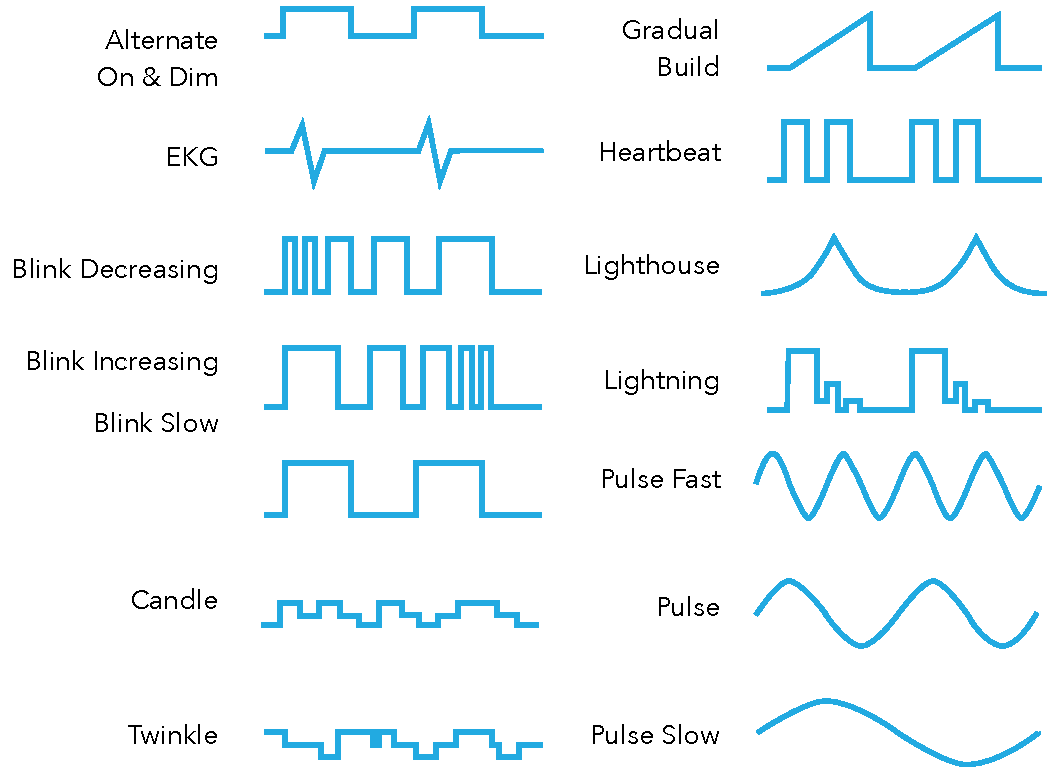
\includegraphics[keepaspectratio, width=0.47\textwidth]{figures/behaviors.pdf}
      \caption{ Example behaviors for point lights, encoded as pulse code modulations. }
        \label{fig:behaviors} 
    \end{figure}

  \textit{Tasks}. We consider a  task $\tau$ to be any set of jobs that causes an actuator $A$ to perform a series of actions.  Thus a  task $\tau_{A, i}$ for actuator $A$ contains a sequence of jobs $J_{A,i,j}$ = $\langle t, I \rangle$, where $t$ denotes the request time and $I$ denotes the PWM signal issued by the $j^{th}$ job of task $\tau_{A, i}$. Tasks are the actuator-level representation of a behavior. We also assume that there exists one job per unit time for a given actuator.

  \textit{Actuators}.
  An actuator with input range $I_r$ is modeled using three types of profiles, hereforth termed the MPS profile, encoded as lookup tables:
  \begin{itemize}
      \item \textit{Mechanical impedance profile} $M(v)$ - this represents mechanical latencies due to structures resisting motion for each $v$ vector (e.g., certain stepper motor requires at least 100ms to go from min to max) 
      \item \textit{Perceptual, or Gamma, profile} $G(P)$ - this represents the conversion from  perceptual magnitudes to PWM signal (e.g., 50\% brightness on an LED [$I_r = [0, 255]$] is equivalent to a ~39 PWM load)
      \item \textit{Software impedance profile} $S(v)$- this represents the software latencies at each for each $v$ vector in PWM signal(e.g., BlinkM introduces a 20ms delay to each  value change) 
    \end{itemize}
    Aside from the perceptual profile, the values must be generated experimentally or derived from manufacturer documentation. We compiled a set of 15 actuators available through our public API. The perceptual profile can be modeled using Equation \ref{stephens_power_law}. 


  \textit{Behaviors}. At the human-level, behaviors $B$ are defined as tasks which semantically convey information and are encoded in perceptual space, as opposed to actuator-intensity space. We encode behaviors as a 12-bit pulse-code modulation (PCM) sampled at 128Hz (Figure \ref{fig:behaviors}. PCM is an uncompressed encoding format regularly used for audio applications, which samples and quantizes analog values at regular intervals. These behaviors were derived from field work conducted by Harrison \textit{et. al.} for point-lights \cite{harrison_unlocking_2012}, as well as from custom built program-by-demonstration interfaces. We represent a PCM signal $W$ as a sequence of tuples $\langle t, P \rangle_i$, where $t$ denotes the sampled time and $v$ denotes the perceptual magnitude issued by the $i^{th}$ sample of the signal.


  Furthermore, we assume the following properties that are currently ubiquitous amongst embedded systems. 

  \begin{itemize}
  \item For any actuator $A$, the WCET of each job has low variance since most processing is offset by hardware components (e.g., internal controller in stepper motors), and thus the WCET of these jobs is I/O bound and regular. However, while this predictability adds more flexibility to scheduling routines, it is important to note that the density of jobs for a task $\tau_i$ can \textit{and often} changes for each period $T_i$ as well as from actuator to actuator.

  \item Another important distinction of a task is that its jobs hold state. Issuing a job at $\langle t=1s, 120 \rangle$ and $\langle t=2s, 120 \rangle$ is redundant since the 120 PWM load persists from $t=1s$ until another command changes its state.
  \end{itemize}

  Lastly, we will be referring to terms and concepts prevalent in psychology literature, however most relevent to the application of a scheduler is the \textit{Just-Noticeable Difference} (JND) which can be conceptualized as a unit measure of perceptual time. Formally, JND is defined as the amount a stimulus must be changed in order for the difference to be detectable at least half the time. 
  This measure is used in experimental psychology to calculate perception of stimulus e.g., lux $\rightarrow$ brightness, amplitude $\rightarrow$ loudness, temperature $\rightarrow$ heat, and has been used by Chaudhary et. al.\cite{chaudhary_perceptual_2001} for perceptual scheduling of audio stimuli. 

  Throughout this paper, our scheduler will be using the JND unit time scale, which is experimentally derived as follows: 
  \begin{enumerate} 
    \item Serially send $n$ equivalent sine-wave tasks to each actuator in the system.
    \item Adjust the period $T_i$ of the sine-wave until all actuators appear \textit{just-noticeably} synchronous to obtain 
    \begin{equation}
      k = \frac{T_i}{n}
      \label{eq:server_u}
    \end{equation}
    \item Repeat trial varying $n$, and report the median value $k$ over all trials. 
    \  
  \end{enumerate}

  For the Arduino UNO atmega328 microcontroller, we report $k = 0.585 ms$, over 10 trials and 5 participants, and a randomly sampled $n$-actuator range of [1-40]. 
  
  Since the ratio of JND/reference has been observed to be roughly constant,  psycho-physicists use the Steven's Power Law formulation to map physical stimulus $I$ to perceptual stimulus $\psi(I)$.
  \begin{equation}
    \psi(I) = kI^a
    \label{stephens_power_law}
  \end{equation}
  Notably, this formulation is used to gamma-correct modern LCD displays; we use this formulation in our system but utilize it to adjust other non-light based modalities. 
  
  % We define a base wave $W$ as a sequence of tuples $\langle t, P \rangle$ gathered \textit{a priori} from content creation routine described in detail in prior work [1]. As an example, the Wpulse has a sine wave as its base representation, oversampled at a regular interval. 


  \subsection{Perceptual Task Compiler}

    The major role of the PT compiler is to convert perceptual-space behaviors into an equivalent actuator-space representation $\tau_A$, conditioned on the type of actuator $A$. 
    Behaviors are encoded at a higher resolution than is needed for mechanical actuators, thus we define a set of filters that can be used to reduce the complexity of the incoming signal, as well as convert to actuator-space. We define the PT transform as $F_A$ on the poset behavior $B$ to yield the poset task $\tau$.  
    \begin{equation}
      F_A(B) = (F_S \circ F_M \circ G)_A (B, \leq) = \tau
    \end{equation}
    The PT function $F_A$ is comprised as the composition of three transforms, derived from the MPS profiles for actuator $A$. 

    The gamma correction transform G is as follows:
    $$ G_{B} = \{P^{1/\gamma} \cdot \frac{\text{max}(I_r)}{\text{max}(I_r)^{1/\gamma}} \vert t, I_r \in B\} $$
    where $\gamma$ is the Stephen's Power Law exponent from Equation \ref{stephens_power_law}, and $I_r$ is the input range for actuator $A$. 

    We then apply the mechanical and software correction transform by first taking the derivative of B: 
    $$ B' = \frac{d}{dt}(G_{B}) = \frac{dI}{dt} = v  $$
    and apply the following filters which drop impossible actuations as defined by the mechanial $M$ and software $S$ profiles.
    $$ F_M(B', \leq)  = \texttt{isDefined}(M(v))$$
    $$ F_S(B', \leq) = \texttt{isDefined}(S(v))$$

    At the conclusion of applying $each$ of these filters, redundant values are removed from $B$ such that $\tau$ is the sparse representation of the original behavior.

    \subsubsection{Admission criteria}
    This software ($S$) and mechanical ($M$) profiles can be used to detect behaviors $B$ that cannot be achieved on actuator $A$. 
    This is used as the admissions criteria by the compiler. Often times, the original behavior can be modified by some time scalar $c$.  We can obtain the maximum and minimum $c$ such that every actuation in $B$ is admissible by taking the ratio of the minumum allowed $v$ in $M$ or $S$ to the minumum $v$ in $B$ : 
    \begin{equation}
    \begin{split}
        c_{\min } =  \frac{\min (B')}{\min (M(v))}
      \end{split}
    \quad
      \begin{split}
       c_{\max } =  \frac{\max (B')}{\max (M(v))}
    \end{split}
    \end{equation}
   
    \subsubsection{Additional metadata}
    We extend the task $\tau_A$ with two additional properties for each job in its sequence. These properties takes into account Gestalt psychology and are applied as a perceptual optimization.
    \begin{itemize} 
    \item \textit{hardness} (h) - a synchronization parameter. Directionality of elements is a main grouping mechanism (e.g., moving elements that are moving in two different directions are perceived as groups). 
    \item \textit{locality} (l) - areas in the fovea, or center of vision, are much more perceptually stringent than peripheral elements. 
    \end{itemize}
  
    The hardness parameter is composed from $B'$, specifically when jobs express a change in direction of the PWM load, i.e., $v$ = 0 or $v = \max(I_r)$. Let the set of directionally shifting jobs be defined as:

    $$v_\text{shift} = \{ i \,\vert \,i, v = 0 \,\text{or} \, v = max(I_r) \in B'\}$$ 

    We also include the first and last job index to $v_\text{shift}$. Each job is assigned a hardness value equal to the inverse of the shortest euclidean distance to a shifting value as follows:
    $$ h_{i} = \frac{1}{\min (\dis(i, v_\text{shift} ))}$$ 
    for the $i^{th}$ job in task $\tau$. As such, large changes in intensity are assigned a higher hardness whereas smooth changes are assigned lower hardness. 

    Lastly, a locality property $l$ is defined based on the physical topology of the actuator system. In our implementation, we defined hand-defined centers of the topology, and assumed a physically static layout. For a more dynamic approach, one can construct a graph and run a centroid-based clustering algorithm. We leave this for future work.  
  
  % END OF DRAFT
  In conclusion, a task $\tau$ consists of a sequence of jobs $J_i = \langle t, I, h, l \rangle$ which is then fed into our perceptual scheduler. 

  \subsection{Perceptual Task Evaluator}
  Using a perceptual model derived from known stimulus power-laws in perception literature, we can use psychophysics method-of-constant-stimulus with human subjects to evaluate the quality of service (QoS) of the perceptual scheduler. However, this is an expensive form of evaluation. 
  We can synthetically evaluate perceptual accuracy as a peak-signal-to-noise calculation (PSNR) from the original PCM behavior $B$ and the output signal $\tau$. We can calculate the total JND units that were lost by converting back from gamma space using $G'$ and sampling the output at the same sampling rate $f$ (128Hz) as the originally encoded $B$. We define the QoS for a task $\tau$ as the sum of lost JND units over the energy of the overall task as follows:
  $$G'(I, I_r) = \frac{\max(I_r)^{1/\gamma}}{\max(I_r)} \cdot (I)^\gamma $$
  \begin{align}
  PSNR(B, \tau) &= 10 \cdot \log_{10} \frac{\max_I}{MSE}\\
  &= 20 \cdot \log_{10} \int_{t_0}^{t_f} \frac{2^k-1}{\sqrt{\lvert\lvert G'(B(t) - \tau(t) \rvert\rvert}}  \, dt
  \label{eq:error}
  \end{align}


  where $k$ is the PCM resolution and $dt = 1/f$. While we can extend this error metric to penalize more for synchronization and other perceptual errors, we use this form to calculate a lowerbound on perceptual error, as opposed to using a more complicated and less general metric. 



  \subsection{Perceptual Scheduler}
  We implemented our scheduler in Python and sent the final schedule through a serial connection to our testbed systems. Actuation behaviors were previously compiled and stored in a SQL database. Although not directly ported onto the embedded system, the current pipeline can be emulated on an embedded system since the serial communication is not the I/O bound, and precompiled behaviors can be loaded from an external memory cache or retrieved from a WiFi module. The cost of running scheduling tasks will increase, but we show that using a CBS scheduler, we can modify the allowed budget that is allocated to the scheduler to allow other system tasks (such as reading sensor values) to operate. 

  The perceptual scheduler is constructed as a CBS scheduler, where each node in the system is modelled as a server $s$ with tuple $\langle Q_s, T_i \rangle$, where $Q_s$ is maximum budget, and $T_s$ is the period of the server. 
  All perceptual tasks $\tau$ are treated as hard tasks, since its WCET is known. 

  \subsubsection{A perceptual baseline - EDF parameters}
  According to Lemma 1 from \cite{abeni_integrating_1998}, a task $\tau$ is EDF schedulable if and only if $C_i \geq Q_S$ and $T_s = T_i$. 

  By assigning $U_s = 1/k$ as derived in Equation \ref{eq:server_u}, we can obtain the EDF parameters ($C_i, T_i$). The maximum budget $C_i$ is equal to the number of job collisions over time, and can be derived by taking the histogram of a task $\tau$ binned on deadline $t$ as follows:
  \begin{equation} 
    C_i = \max(\text{hist}(\tau, t))
    \label{eq:collisions}
  \end{equation}
  with a period equal to $T_i = C_i / U_s$. 

  For a $n$-node server where each actuator node is sent identical tasks, at least $n \cdot k$ ms are needed to actuate the nodes perceptually synchronous, and no more than a budget of $n$ is needed.   

  \subsection{Schedulability test}
  In order to prevent speed up effects when scheduling soft tasks, a known technique for CBS schedulers is to use a skip strategy: when a job finishes after its absolute deadline, the next job is skipped. This strategy violates our guarantees for synchronization. As such, perceptual tasks must be treated as hard tasks. 

  \begin{theorem}
     Let H be the set of identical hard task $\tau$  sent to each actuator $A_i$ in a $n$-actuator system. Given that the WCET of each job in $\tau$ is $k$, then H is only schedulable if CBS is EDF-reducible with parameters ($Q_s, T_s$) where
     $Q_s \ge \max(\text{hist}(\tau, t))$, and $T_s \ge Q_s / U_s $. 
  \end{theorem}


  \begin{proof}
    A set of hard tasks are considered EDF schedulable \cite{xu_scheduling_1990} if: 
    \begin{equation}
      U = \sum_{i=1}^n \frac{\text{WCET}(J_i)}{T_i} \leq 1
    \end{equation}
    for $n$ processes. Since $\text{WCET}(J_i) = k$ and since each task $\tau$ has identical $T_i$ = $T$, this results in an schedulability test of $n \cdot k \leq T$.

    Given that $T_i = C_i / U_s$ \cite{abeni_integrating_1998} and CBS($Q_s, T_s)$, we prove by contradiction: 
    \begin{align*}
      n \cdot k &> T\\
           &> C_i / U_s \\
           &> \max(\{\text{hist}(\tau, t) \vert \tau \in H \}) \cdot k \text{ (Equation } \ref{eq:collisions})\\ 
           &\ngtr n \cdot k
    \end{align*}
    Therefore, H is schedulable if CBS is EDF reducible. 
  \end{proof}

  As such, degradation of the perceptual signal occurs when these EDF constraints are not satisfied. A CBS server with these EDF parameters serves as a baseline where every job is guaranteed to be schedulable. 

  \subsection{Perceptual saliency queue}
  As an optimization, we change the enqueue routine for the CBS algorithm from a FIFO, to a priority queue that can be used to model saliency within the perceptual system. Within each quanta, jobs are assigned the following priority:

  $$ J.priority =  (1 - \frac{1}{J.l}) + 10 \cdot \frac{1}{J.h} + 1000 \cdot J.$$

  where a job closer to a perceptual center (locality $l$) has a higher priority, tie broken by jobs that have directional changes in intensity (hardness $h$), and finally resolved by the earliest deadline $t$. By Equation \ref{eq:server_u}, the top $Q_s$ jobs are accepted, and the rest are placed into the temporal dithering routine. 

  \subsection{Temporal dithering}
  In order to increase the CBS capacity and scale the number of nodes in a system, we extend the CBS algorithm to schedule jobs which failed the schedulability test, hereforth termed rejected jobs, in quanta with available budget, however we modify the job dependent on it new quanta location. We accomplish this through a technique temporal dithering as detailed in Algorithm \ref{alg:dithering}. 

  

\begin{algorithm}
 \KwData{Let $J_r$ be a job from the task $\tau$ rejected from quanta $q_r$, with closest available quanta $q_C$ at time $CT$. Let $J_N$ as the nearest job in the $\tau$ sequence scheduled in quanta $q_N$ at time $NT$.}

 \For{$J_R$ in rejected\_jobs }{
  \If{$\neg J_{\text{close}}$}{
    delete $J_R$\;
    return\;
  }
   d = $\lvert\lvert N - C \rvert\rvert$\;
   pos = $C + d$\;
  \eIf{$C = N$}{
   $J_N :=$ lerp( $J_R, J_N, pos, d$)\;
   delete $J_R$\;
   }{
   $J_{\text{R}} :=$ lerp( $J_R, J_N, pos, d$)\;
   $q_i$.enqueue($J_R$)\;
  }
 }

 \caption{Temporal Dithering}
 \label{alg:dithering}
\end{algorithm}





 

  \section{EVALUATION}
  In order to evaluate or scheduling mechanism, we used the Perceptual Task Evaluation (PTE) metric (Equation \ref{eq:error}) to simulate perceptual accuracy. We define four different schedulers to observe the full effect of each portion of the pipeline: Earliest Deadline First (\schedule{EDF}), Constant Bandwith Server with skip (\schedule{CBS-S}), and the Perceptual Scheduler (\schedule{PS-A}) without saliency queue, and the full-featured Perceptual Scheduler (\schedule{PS-T}). 

  Ultimately performance of our system will be evaluated experimentally through a JND psychophysics experiment. That is, given a set of perceptual tasks on a $n$-node system, does a user notice a lapse or abnormality in the output? The microbenchmarks we chose will focus on finding the conditions where a user may see such a lapse or degradation of quality. Although we do not conduct a user study in this paper, the results from the the PTE metric has correlated well with output from our experimental setup. We leave the human evaluation for future work. 

    \begin{figure}[t]
      \centering
      
\includegraphics[keepaspectratio, width=0.47\textwidth]{figures/testbed.pdf}
      \caption{ A testbed system consisting of 38 actuators, each individually controlled by a 16 MHz atmega328 micro controller (Arduino Uno, $Q_s = 10$) through a 12-bit PWM $\text{I}^2$C interface (PCA9685). }
      \label{fig:testbed} 
    \end{figure}
  \subsection{Testbed - 38-node system}
  A testbed system (Figure \ref{fig:testbed} was constructed using a 16 MHz atmega328 micro controller (Arduino Uno) modified with three 16-channel 12bit PWM I2C drivers (PCA9685), for a total output capacity of 48 actuators. Our prototype consisted of 32 LEDS (8R, 8Y, 16G) and 5 micro servos (TowerPro SG90). Alternative testbeds were constructed to prove the feasibility of other actuator modalities (e.g., steppers, heatpads), although these were not added to the final system. 

  %   \subsection{Types of actuators used}
  % \begin{itemize}
  %   \item Light: LED, BlinkM MaxM (COM-09000)
  %   \item Motion: Binary solenoid, Stepper, brushless, erratic vibration, and servo motors 
  %   \item Heat: 5x15cm Heatpads (COM-11289)
  %   \item Sound: Piezo (SEN-10293)
  % \end{itemize}
  
  As depicted in Figure \ref{fig:system}, behaviors were stored on an external server, which would then be perceptually compiled. While we have only one node in our envisioned distributed network of actuator components, we anticipate that devices will propagate instructions similar to current sensor streaming techniques. Global clock synchronization is necessary to provide a seamless experience; for this reason, we use the tunable parameters $Q_S$ of our \schedule{PS-T} scheduler which we show below can be adjusted to fit the performance of different types of hardware, degrade gracefully, and still enforce deadlines. 


  \subsection{Microbenchmarks}
  In our survey of actuator behaviors in interactive devices, we noted three characteristics of behaviors: 
    \begin{itemize}
    \item Synchronicity - behaviors were either intended to synchronize with each other, or propagate through the system (e.g., follow-the-leader, burst).
    \item Discrete/smooth - some behaviors require discrete shifts in intensity (e.g., SOS), while others follow a smooth curve (e.g., lighthouse). 
    \end{itemize}

  As such, we developed a (2x2) microbenchmark factorial design evaluated on a CBS scheduler and the PTS scheduler on a heterogeneous configuration --- the system is composed of multiple types of actuators. 

  \pagebreak
  \subsection{Results - Microbenchmarks}
  The result from the microbenchmarks are display varying number of actuators (Figure \ref{fig:pulse_actuators}) and varying the budget alloted to each quanta (Figure \ref{fig:micro_system}). The graphs show a consistent improvement over the CBS scheduler. 

  From these experiments, we noted a potential drawback of the PSNR error metric. PSNR penalizes on overall energy, and not for shifts in energy. For example, for $n > 30$, the graphs plateau at around 7.3dB. This is due to the fact that since an actuator holds state, it can hold a constant intermediate value, cause a mean-square error to register noise.

  Also, a particular abberation occurred for the staggered pulse behavior benchmark. When $n$ > 30, the pulse behavior resonated on its Nyquist frequency, causing an increase in quality.




  \begin{figure}[t]
      \centering
      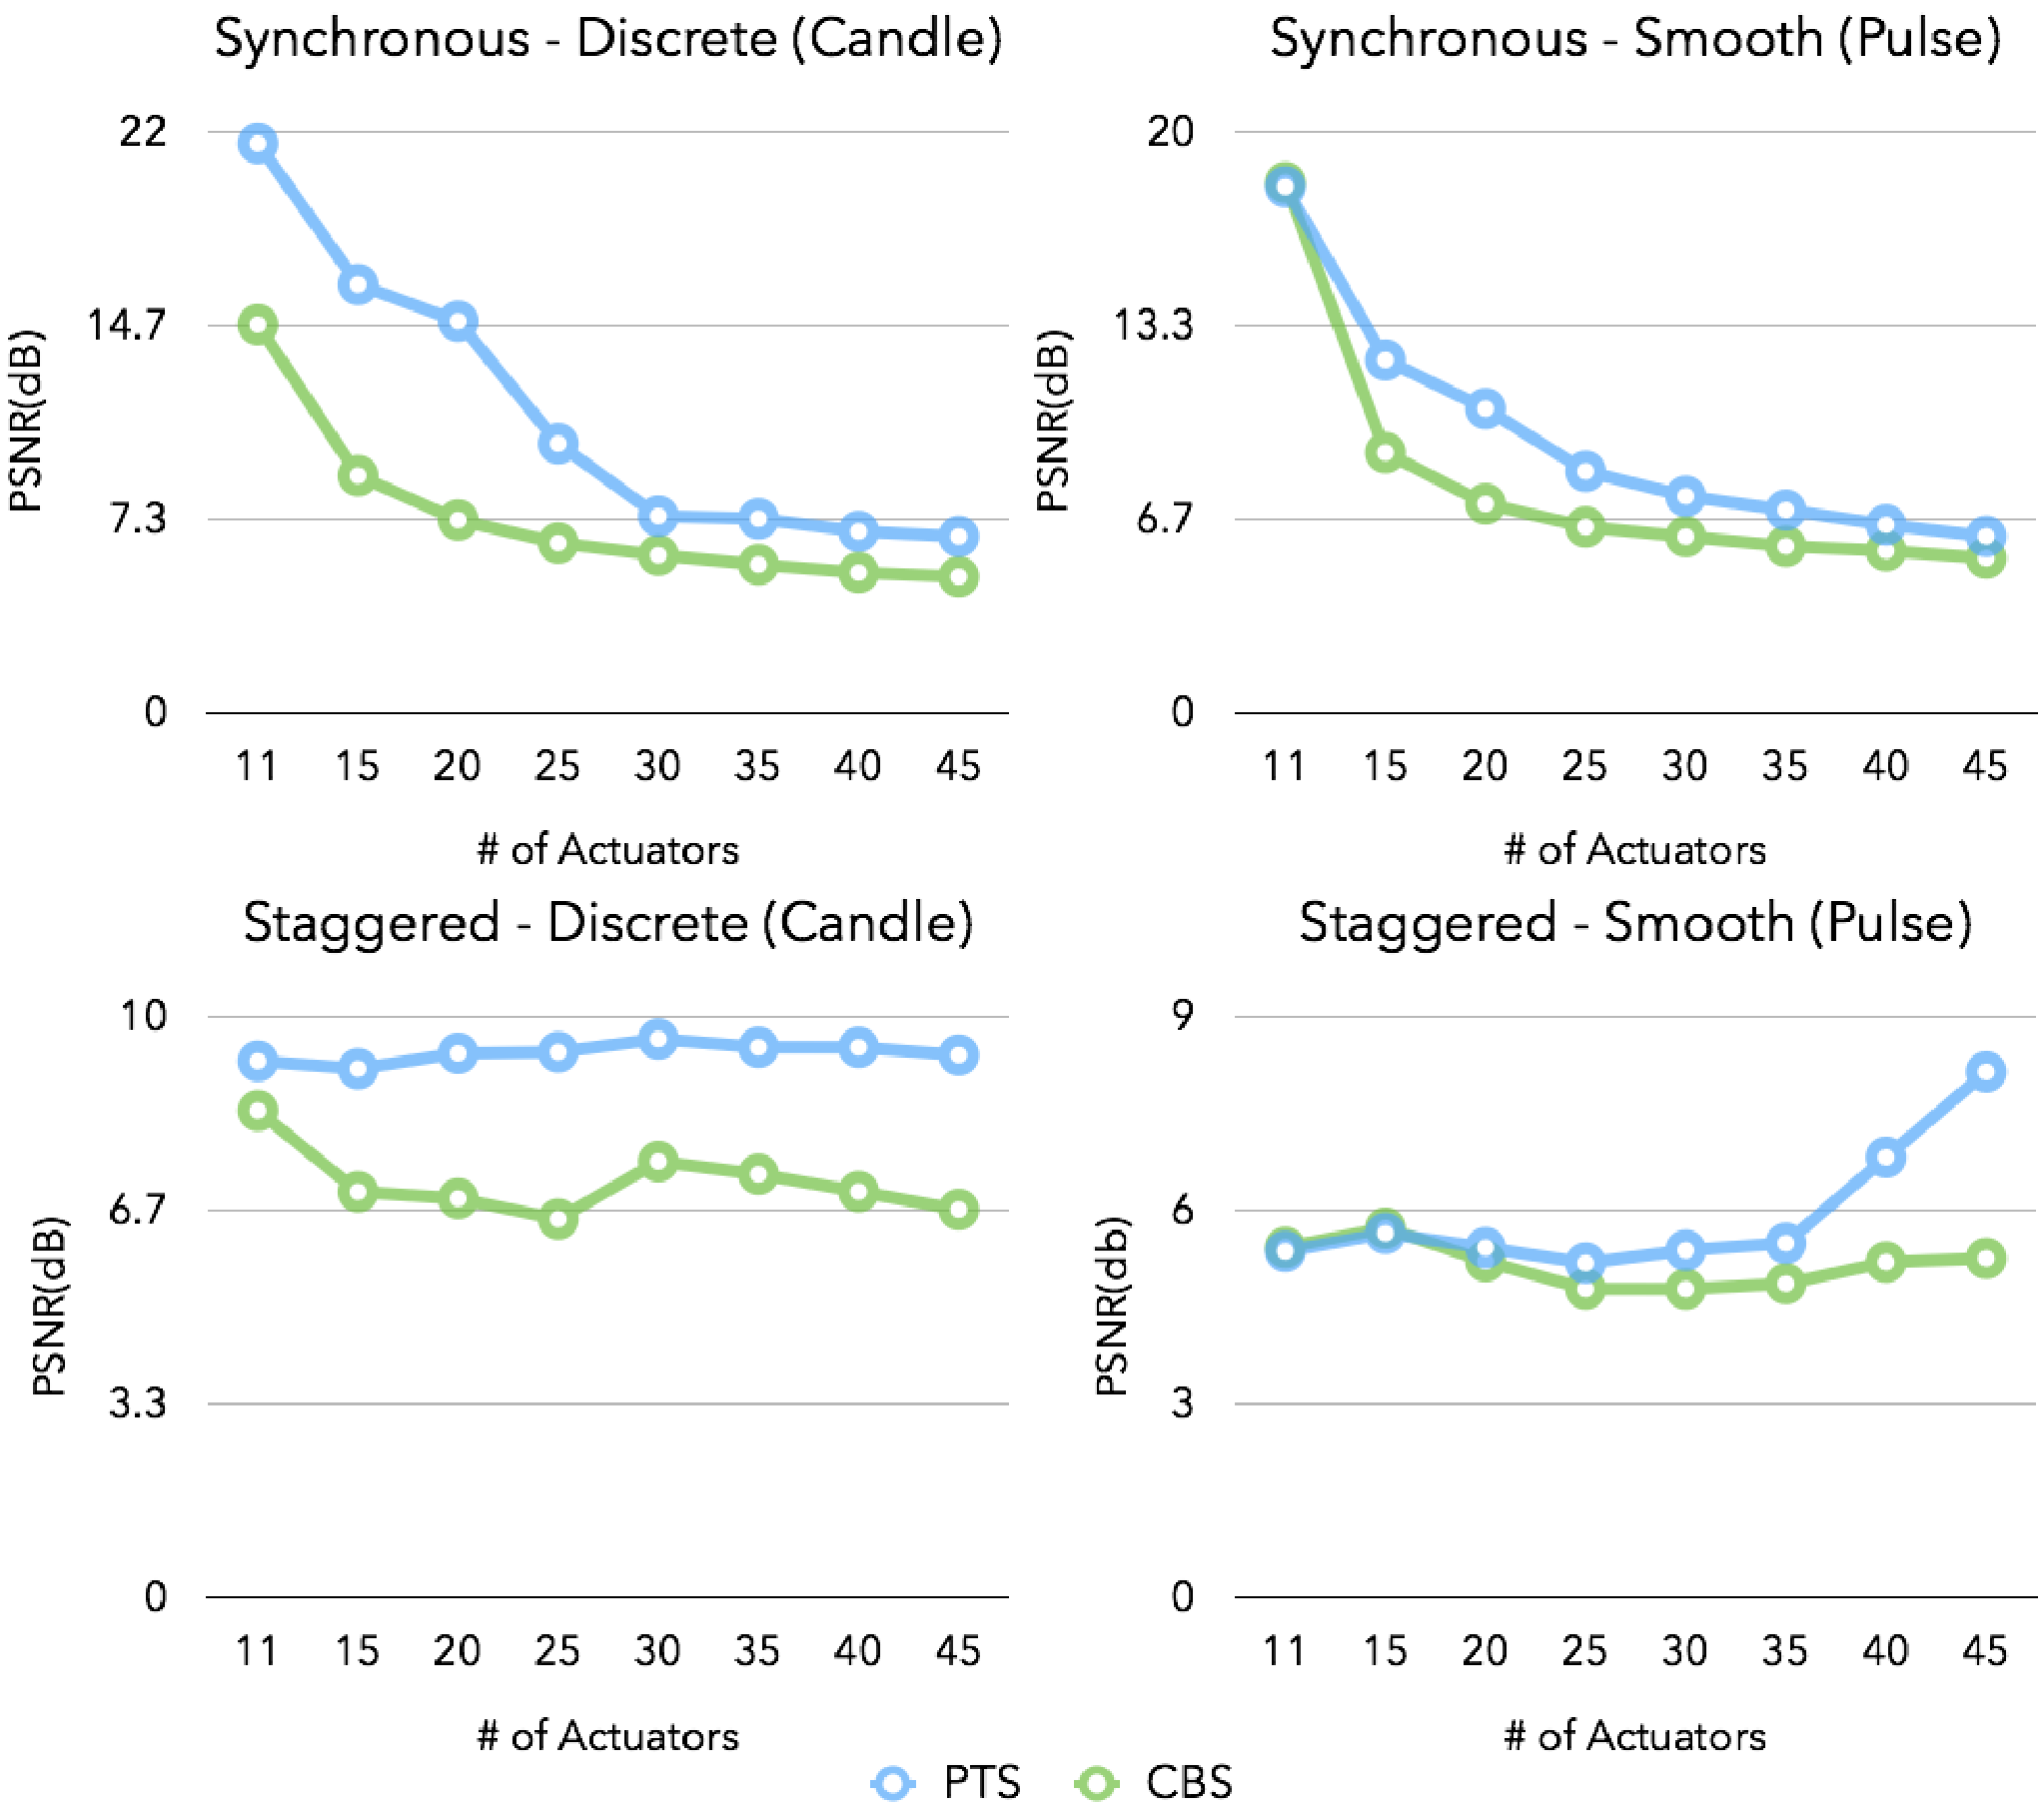
\includegraphics[keepaspectratio, width=0.47\textwidth]{figures/pulse_actuators.pdf}
      \caption{ Microbenchmark tests altering the number of actuators in the system. These results were simulated in a budget (Qs = 10) on a heterogenous system. The top row displays synchronous commands to each actuator in the system, while the bottom displays staggered commands (on a 1ms time step). Larger PSNR values indicates better quality of service.  }
        \label{fig:pulse_actuators} 
    \end{figure}

     \begin{figure}[t]
      \centering
      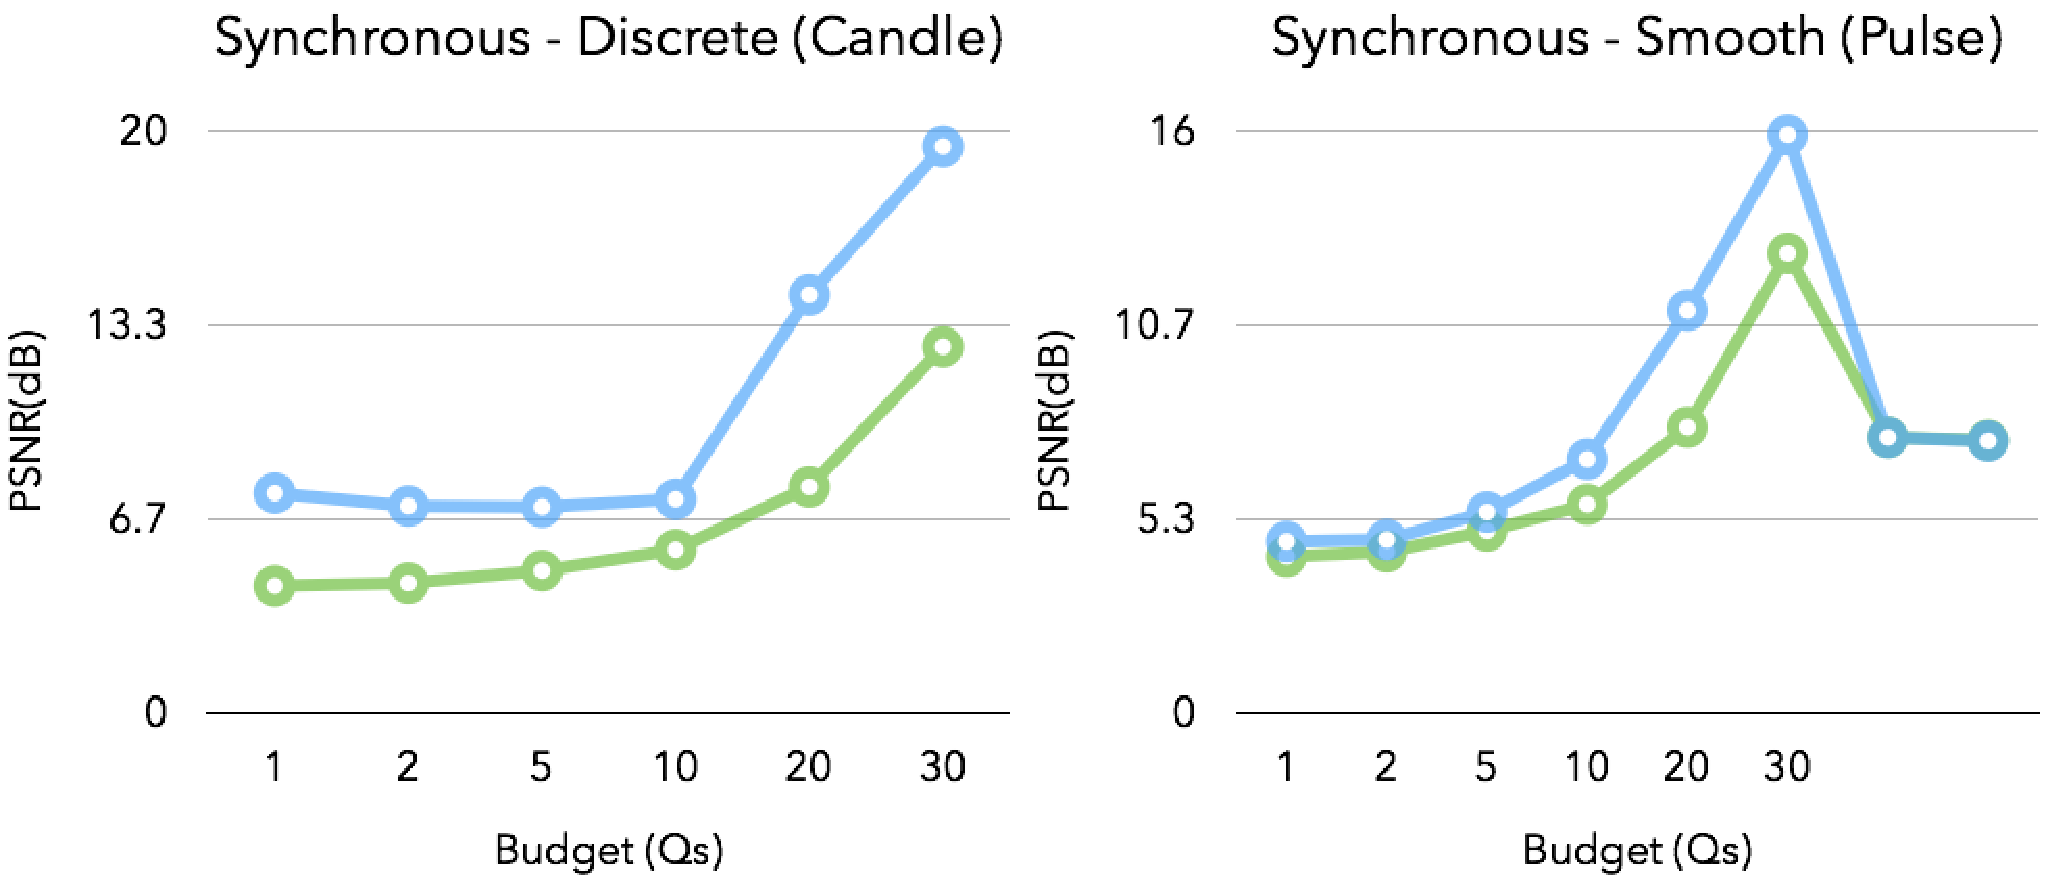
\includegraphics[keepaspectratio, width=0.47\textwidth]{figures/micro_system.pdf}
      \caption{ Microbenchmark tests altering the budget allocated to the system.  These results were simulated in n = 35 node heterogenous system. The top row displays synchronous commands to each actuator in the system, while the bottom displays staggered commands (on a 1ms time step). Larger PSNR values indicates better quality of service.  }
        \label{fig:micro_system} 
    \end{figure}

    \subsection{Macrobenchmarks}
  In this section, we describe synthetic macrobenchmarks devloped to evaluate the system. Since actuation behaviors within distributed systems have not been fully developed, we emulate the same behaviors found in centralized multi-actuator systems. 

  Our example system is a theatre complex, which is composed of a projector, an eight-channel surround sound system, sixteen overhead lights, two lines of track lighting running the length of the complex, two exit signs, and a fire alarm. The behavior was composed in the context of a fire evacuation drill. The situation is marked in Figure \ref{fig:macro} with the following events. The benchmark begins in a \schedule{IDLE} stage – projector and audio system are on running at 30fps; the track lighting over overhead lights fade to begin the feature film. It then progresses to a \schedule{ALERT} stage, the alarms turns on, turning off the projector and sound, and pulsing a danger message through the track lighting. Finally, it enters an \schedule{EXIT} stage – the track lights begins to propagate a signal towards the exit doors. Exit lights are then pulsing for a five minute period. 


  \subsection{Results - Macrobenchmark}
  We ran our perceptual scheduler against a CBS scheduler, with a skip strategy. This resulted in an EDF behavior where periods with full utilization rejected tasks that overspent the allotted budget. The schedules were evaluated as time-signals, where logs were kept for commands sent to each actuator. These commands were reconstructed, and integrated at a supersampled rate to obtain the JND error. 
  For the macrobenchmark report a PTS PSNR of 11.0574422702, and a CBS PSNR of 10.8947625321.
  We anticipate that this slight difference is due to the confounding effects of the PSNR metric and leave for future work a evaluation metric that penalizes missteps. 


  \section{Future Work}
  Also, while our current Gestalt marking technique for high-priority jobs does aid in the perception of synchronization, certain behaviors such as ones with random elements, are corrupted by this optimization. A user could define higher-order semiotic points along the tasks that demarcate important synchronization areas. 

  Currently, we have behaviors developed for light and angular motion. However, more extreme actuation profiles, such as those from a heat pad, could introduce some additional variables into our PT compiler. We anticipate testing the extendability of the PT compiler under heat, tone, and vibration in the future. 

  Lastly, our approach currently experimentally evaluate on a single controller system. While we have only one node in our envisioned distributed network of actuator components, we anticipate that devices will propagate instructions similar to current sensor streaming techniques. Global clock synchronization is necessary to provide a seamless experience, and and as such the system will likely need to account for clock skew. 

 \section{Limitations}
  Our current evaluation metric, while taking into account the human perceptual system, is incomplete without a formal user study. In the audio perceptual scheduler, Chaudhary utilized a 5-point Likert scale evaluation to quantify the perceived loss of quality \cite{chaudhary_perceptual_2001}. We anticipate using a similar technique to evaluate the quality of service of the scheduler. 

  A major limitation of our work is that we do not take into account audio actuation. Since this is a major area of study, and the most diverse of the modalities, we excluded it from our scheduling mechanism. However, incorporating a synchronized audio routine is certainly necessary to complete the scheduler for use by industrial and interactive device designers.


  \section{CONCLUSION}
  In this paper, we showed that physical coordinated stimuli require a different metric of performance. Factoring in perception literature, we create a perceptual compiler which converts perceptual tasks, which are highly dependent on the type of actuator used to output them, into uniform tasks which produce correct actuator instructions and perceptually equivalent output. Building off the work of the CBS algorithm, we show that are scheduler can operate on a fraction of the total allowed bandwidth.  Over previous fair-allocation schedulers, we show that our PT scheduler is able to maintain a higher perceptual performance (70\% - 99\%) running on a conventional atmega328 microcontroller on a 38-node system. We also show through simulation that the PT scheduler allows control of up to an orders of magnitude more actuators with an acceptable loss of quality. 


  \section{ACKNOWLEDGMENTS}
  A large part of the content database was made available by Jasper O'Leary, Kenny Wang, and Allen Li, as well as a review of psychophysics literature by Akhila Raju. We also thank John Kubiatowicz for his helpful suggestions on evaluating the system, and Tim Campbell for his aid in the intial formulation of this project.  
\bibliographystyle{acm-sigchi}
\bibliography{expresso}
\end{document}
